\documentclass{standalone}
\usepackage{tikz}
\begin{document}

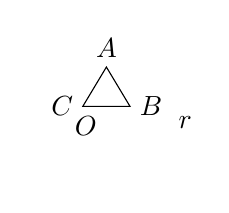
\begin{tikzpicture}
    % Draw the unit circle with white fill
    \fill[white] (0,0) circle (1);
    % Draw the triangle with one corner pointing upwards
    \draw[black] (0,0.5) -- (0.3,0) -- (-0.3,0) -- cycle;
    % Add math labels
    \node at (0,0) [below left] {$O$}; % Center
    \node at (1,0) [below] {$r$}; % Radius
    \node at (0,0.5) [above] {$A$}; % Top vertex
    \node at (0.3,0) [right] {$B$}; % Right base vertex
    \node at (-0.3,0) [left] {$C$}; % Left base vertex
\end{tikzpicture}

\end{document}